\documentclass[lettersize,journal]{IEEEtran} %这一行的作用是设置论文的格式,letterpaper表示纸张大小为美国信纸,journal表示论文类型为期刊论文,IEEEtran表示论文的格式为IEEEtran
\usepackage{amsmath,amsfonts} %这两个包分别是数学公式和数学字体的宏包
\usepackage{algorithm}
\usepackage{algpseudocode}
% \usepackage{algorithmic} %这个包是算法的宏包
\usepackage{array} %这个包是表格和数组的宏包
\usepackage[caption=false,font=normalsize,labelfont=sf,textfont=sf]{subfig} %这个包是子图的宏包,它可以让你在一个图形环境中放置多个图形,可以对子图进行编号,可以对子图进行交叉引用,可以对子图进行标题设置
\usepackage{textcomp} %这个包是对文本模式下的符号进行扩展的宏包
\usepackage{stfloats} %这个包是控制双栏浮动图形和表格的宏包
\usepackage{url} %这个包是对网址进行扩展的宏包
\usepackage{verbatim} %这个包是对抄录环境进行扩展的宏包
\usepackage{graphicx} %这个包是对图形进行扩展的宏包
\hyphenation{op-tical net-works semi-conduc-tor IEEE-Xplore} %这一行的作用是设置英文连字符,可以防止英文单词在换行时过长
\def\BibTeX{{\rm B\kern-.05em{\sc i\kern-.025em b}\kern-.08em
    T\kern-.1667em\lower.7ex\hbox{E}\kern-.125emX}} %这一行的作用是定义BibTeX的标志,这个标志在参考文献中会用到
\usepackage{balance} %这个包是平衡双栏文档最后一页的双栏高度的宏包



\begin{document} %这一行的作用是开始论文的正文部分
\title{GraphCPP: A Data-Driven System for Concurrent Point-to-Point Queries in Dynamic Graphs} %这一行的作用是设置论文的标题
\author{IEEE Publication Technology Department %这一行的作用是设置论文的作者
\thanks{Manuscript created October, 2020; This work was developed by the IEEE Publication Technology Department. This work is distributed under the \LaTeX \ Project Public License (LPPL) ( http://www.latex-project.org/ ) version 1.3. A copy of the LPPL, version 1.3, is included in the base \LaTeX \ documentation of all distributions of \LaTeX \ released 2003/12/01 or later. The opinions expressed here are entirely that of the author. No warranty is expressed or implied. User assumes all risk.}} %这一行的作用是设置论文的作者的单位和邮箱,这里的\thanks是设置脚注的命令

\markboth{Journal of \LaTeX\ Class Files,~Vol.~18, No.~9, September~2023}%这一行的作用是设置论文的页眉
{How to Use the IEEEtran \LaTeX \ Templates} 

\maketitle %它和title的区别是,title只是设置论文的标题,而maketitle是使论文的标题和作者的信息生效

\begin{abstract} %这一行的作用是设置论文的摘要
With the widespread application of graph processing techniques in areas such as map navigation and network analysis, there is a growing demand for high throughput in handling numerous point-to-point query tasks concurrently on the same underlying graph. However, existing graph query systems have primarily focused on optimizing the speed of individual point-to-point queries. When it comes to concurrent graph computations, these systems suffer from poor overall throughput due to redundant data access overhead and computational costs.

We observe that due to the power-law distribution characteristic of graph data, the traversal paths of different queries often overlap on local paths composed of a small number of high-degree vertices, demonstrating the data similarity of concurrent point-to-point query tasks. This inspires us to propose a data-driven concurrent point-to-point query system - GraphCPP. It employs a partitioning approach to organize the graph structure data into LLC-level blocks. A key feature is the prioritized loading of active blocks, determined by the number of associated active vertices. This loading strategy, by focusing on active blocks, is instrumental in facilitating concurrent execution of associated query tasks. The outcome is enhanced data sharing and improved data access efficiency. Additionally, GraphCPP incorporates a core subgraph mechanism, which plays a critical role in promoting computational sharing. This mechanism is dedicated to pre-calculating distance values between high-degree vertices within the graph. This pre-calculation enables the rapid determination of distance values for frequently shared path segments when queries are initiated. In this way, it expedites the convergence of query results while optimizing computational sharing. Furthermore, GraphCPP employs predictive techniques during task scheduling to harness data similarity within concurrent point-to-point query tasks effectively. By batching and selecting similar tasks from the task pool, it maximizes the utilization of data similarity. We compare GraphCPP with state-of-the-art point-to-point query systems, including SGraph[x], Tripoline[x], and Pnp[x]. Experimental results demonstrate that GraphCPP improves the efficiency of concurrent point-to-point queries by a factor of xxxx  
\end{abstract}

\begin{IEEEkeywords}
Class, IEEEtran, \LaTeX, paper, style, template, typesetting.
\end{IEEEkeywords}


\section{Introduction}
\IEEEPARstart{P}{oint-to-point} query tasks on graphs refer to the exploration of a specific relationship between two objects utilizing the graph as a universal data structure. Unlike traditional graph query methods, point-to-point queries on graphs specifically analyze the associations or paths between two specific vertices, without the need to consider complex queries involving the entire graph or its large-scale subsets. This targeted querying strategy endows point-to-point queries with significant optimization potential. For certain versions of monotonic graph query algorithms, such as Point-to-Point Shortest Path for SSSP (PPSP), Point-to-Point Widest Path for SSWP (PPWP), and Point-to-Point Narrowest Path for SSNP (PPNP), specific path attributes between two vertices can be accurately determined without the need for or with minimal querying and processing of unrelated other vertices or edges. Due to the efficiency of point-to-point queries in graph analysis, it has found extensive practical applications in various fields. For instance, in logistics and transportation, finding the shortest path between two locations; in social network analysis, recommending potential friends to users by examining the relationship chain between two users; in financial risk analysis, analyzing how risks propagate from one entity to another; these popular applications have raised the demand for executing large-scale concurrent point-to-point queries on the same underlying graph. 

However, existing solutions for point-to-point queries have focused on accelerating the efficiency of individual queries, overlooking optimization for concurrent queries. To achieve concurrent point-to-point queries, the following two challenges need to be addressed.

Firstly, achieving data sharing is imperative. There exists significant overlap in the traversal paths of different query tasks. However, under the existing execution paradigm, data isolation between concurrent tasks prevents the sharing of overlapping data, resulting in redundant data access. Additionally, different tasks exhibit varying access sequences for the same graph structure data, further complicating the facilitation of data sharing.

Secondly, enabling computational sharing is crucial. Graph data often adheres to a power-law distribution, where segments formed by a small number of high-degree vertices frequently appear in the shortest paths of different queries. Due to the abundance of neighboring vertices surrounding high-degree vertices, repeated traversals by different tasks often lead to an explosive growth in computational costs. Some existing systems have attempted to employ global indexes for computational sharing, incurring substantial costs in computation, storage, and updates. This approach limits the coverage and precision of computational sharing.

In response to the previously mentioned challenges, we introduce GraphCPP, a data-driven system tailored for concurrent point-to-point queries on dynamic graphs. To address the issue of data sharing among concurrent tasks, we present a data-driven caching execution mechanism that shifts from the conventional "task→data" scheduling approach to a "data→task" strategy. This change allows for concurrent access to graph structure data across multiple tasks. Under this execution paradigm, GraphCPP initially determines the order of data scheduling, dividing graph structure data into fine-grained blocks at the LLC level. Subsequently, it associates each query task with the relevant graph block based on the block where the active vertex set of the task resides. As the active vertices change in each round, the number of associated tasks for shared blocks is updated accordingly, with blocks having more associated tasks being given higher scheduling priority. To implement the "data→task" scheduling approach, GraphCPP utilizes an associated task triggering mechanism. It prioritizes the loading of graph blocks into the LLC and utilizes task-data association information obtained in each round to trigger batch task execution associated with the current block, enhancing efficient access to shared data. In response to the challenge of computational sharing, GraphCPP introduces a query acceleration mechanism based on core subgraphs. It streamlines the traditional "global index," which maintains distance values for all vertices, into a "core subgraph index" that exclusively maintains distance values between high-degree vertices. The core subgraph effectively creates direct edges between interconnected high-degree vertices, representing the shortest distance between them. When querying a high-degree vertex, the program can access all other high-degree vertices, similar to visiting neighboring nodes, enabling computational sharing across overlapping paths. The streamlined core subgraph index incurs significantly lower overhead than the global index, allowing for the inclusion of more high-degree vertices in the core subgraph. This expands the coverage of frequently shared paths, ultimately enhancing computational sharing performance. Additionally, by predicting the traversal paths of different query tasks, we prioritize batch task execution for tasks with substantial overlap, further optimizing the performance of concurrent queries.

This paper makes the following contributions:
\begin{enumerate}
  \item{Analyzed the performance bottleneck caused by redundant data access in existing point-to-point query systems when handling concurrent point-to-point query tasks. Proposed leveraging data access similarity among concurrent query tasks to optimize concurrent task throughput.}
  \item{Developed GraphCPP, a data-driven concurrent point-to-point query system on dynamic graphs, achieving data and computational sharing among concurrent tasks. Additionally, introduced a strategy for batch execution of similar tasks.}
  \item{We compared GraphCPP with the state-of-the-art point-to-point query system XXXXXX. The results demonstrate XXXXXXXXXX.}
\end{enumerate}

\section{BACKGROUND AND MOTIVATION}
Existing solutions have primarily focused on accelerating the speed of individual queries. For instance, PnP employs a lower-bound-based pruning method to reduce redundant access during the query process. Tripoline maintains a daily index from the central vertex to other vertices, enabling rapid queries without prior knowledge. SGraph leverages the principle of triangular inequalities and proposes a "upper bound + lower bound" pruning method, further reducing redundant access during point-to-point query processes. However, as shown in Figure x, our statistics indicate that concurrent point-to-point queries on graphs are becoming an increasingly pressing demand. They prioritize the throughput of concurrent query tasks and are more tolerant of the speed of individual queries. As depicted in Figure x, we demonstrate that existing systems exhibit poor throughput when handling large-scale concurrent queries. This undesirable outcome arises from the substantial redundant data access between concurrent tasks. To qualitatively analyze the aforementioned issues, we conducted performance evaluations of parallel point-to-point queries on XXXXX (machine configurations) using XXXXX (existing best practices) on XXXXX (graph dataset).

This chapter is divided into three parts. We first introduce some concepts in concurrent point-to-point queries. Next, we analyze the performance bottlenecks of current point-to-point query schemes when handling concurrent tasks. Finally, we present the insights obtained from our observations and analysis.
\subsection{Preliminaries}
Definition 1: Graph. We represent a directed graph as $G=(V,E)$, where V is the set of vertices and E is the set of directed edges composed of vertices in V (edges in an undirected graph can be split into directed edges in two different directions). We use $|V|$ and $|E|$ to respectively denote the number of vertices and edges.

Definition 2: Graph Partition. We use $P_i=(V_{P_i},E_{P_i})$ to denote the i-th graph partition of a directed graph, where $V_{P_i}$ represents the set of vertices in the graph partition, and $E_{P_i}$ is the set of directed edges composed of vertices in $V_{P_i}$. In a distributed system, different machine-specific graph partitions $P_i$ are distinct. We partition the graph using edge cuts, where the same vertex may appear on different computing nodes, but there is only one primary vertex, while the others are mirror vertices.

Definition 3: Point-to-Point Query. We use $q_i=(s_i,d_i)$ to represent the query corresponding to task i. Here, $s_i$ and $d_i$ respectively denote the source and destination vertices of query $q_i$. The result value obtained by query $q_i$ is represented as $R_{s,d}$. For different algorithms, it holds different meanings. For example, for shortest path queries, $R_{ib}$ represents the shortest path between $s_i$ and $d_i$. We use $Q={q_1,q_2,\ldots,q_{|Q|}}$ to represent the set of concurrent point-to-point queries, where $|Q|$ denotes the total number of queries.

Definition 4: Index: An index records the distance from one vertex to other vertices and achieves computational sharing by calculating frequently accessed paths. Global Index: We select the top k vertices with the highest degrees in the graph as index vertices $h_i$ (where $i\in [1, k]$, and users can specify k according to their needs, typically set to 16). In this context, $d_{i,j}$ (where $v_j\in V$) represents the distance from index vertex $h_i$ to any vertex $v_j$ in the graph. If there is no reachable path between two vertices, the value is set to an extremely high value. Similarly, $d_{j,i}$ (where $v_j\in V$) represents the distance from any vertex $v_j$ in the graph to the index vertex $h_i$. In undirected graphs, $d_{i,j}$ and $d_{j,i}$ are equal. The creation of this global index is designed to meet specific requirements. Core Subgraph Index: We choose highly connected vertices $h_j$ in the degree range (k, m) to establish a core subgraph index (where $j\in (k, m]$, and users can specify m based on their requirements, typically one order of magnitude larger than k).

Definition 5: Upper Bound and Lower Bound: In point-to-point queries, the upper bound (UB) represents the known shortest distance value from the source vertex to the destination vertex. The lower bound (LB) for the current vertex v to the destination vertex is a conservative estimate of the shortest distance. The predicted LB is less than or equal to the actual shortest distance from vertex v to the destination vertex. According to the triangle inequality on the graph, if a path's distance is greater than UB or if adding the value of LB makes it greater than UB, then this path is certainly worse than existing paths and should be pruned. The values of upper and lower bounds need to be derived with the help of an index. Essentially, they are a form of computation sharing.

Definition 6: Core Subgraph. Similar to an index, a core subgraph also identifies highly connected vertices in a graph, but it employs a lower threshold for selection, which means that more vertices can be chosen. These highly connected vertices form the core subgraph, where the edge weights between two high-degree vertices represent the distance values between the two points. If two vertices are ultimately unreachable, the edge weight is set to a very large value. The key distinction between the core subgraph and a global index is that the core subgraph only maintains indices among high-degree vertices and does not store distance values for reaching non-high-degree vertices.

\subsection{Redundant Computational Costs in Concurrent Tasks}
Due to the characteristics of power-law distribution in graphs, a small number of high-degree vertices are connected to the majority of edges. Therefore, as illustrated in Figure 5, even though high-degree vertices represent only a fraction of the total vertices (XX\%), they appear in a significant proportion of paths (XX\%). Further analysis, as shown in Figure 6, reveals that a substantial portion of the overlapping path data accessed by different tasks consists of high-degree vertices. This implies that different query tasks repetitively traverse the shortest paths between high-degree vertices. Within a single graph snapshot period, the query paths between high-degree vertices remain constant, making the redundant computation for them unnecessary. Additionally, since high-degree vertices have numerous outgoing and incoming edges, computing the shortest paths between them results in substantial computational load. Some existing solutions attempt to establish a global index to reduce redundant computation for different tasks. However, as demonstrated in Figure 7, a global index faces a trade-off between the coverage of vertices in the graph and the inherent overhead of the index. Specifically, when the number of indices is low, the index covers fewer paths, failing to achieve a high level of sharing. When the number of indices increases, the associated computational, storage, and maintenance costs escalate proportionally, diminishing the benefits of the index. Given the variations in the properties of different graph datasets and the evolving scenarios of concurrent queries, determining an optimal number of indices becomes challenging. Consequently, a global index is unable to effectively resolve the issue of computational redundancy

\subsection{Our Motivation}
Based on the above observations, we have gained the following insights:

Observation 1: There is data access similarity among different tasks, and a significant portion of their traversal paths overlap. However, due to the varying times at which different tasks access overlapping data, and the fact that existing point-to-point query systems do not support data sharing among tasks, accessing overlapping data results in redundant overhead. This inspires us to develop an efficient fine-grained data sharing mechanism. By enabling different tasks to share access to the same data at different times, we aim to reduce data access overhead and improve the throughput of concurrent queries.

Observation 2: Segments of paths composed of high-degree vertices are more likely to be repeatedly traversed by different tasks. Different query paths can be visualized as distinct lines, with high-degree vertices acting as intersections of these lines, frequently appearing in various tasks. Existing global indexing methods incur substantial costs and often impose restrictions on the number of indexed vertices, resulting in a low percentage of shareable paths. This insight motivates us to achieve better computational sharing through lightweight indexing.


\section{GraphCPP Overview}
To enhance the execution efficiency of concurrent point-to-point queries on dynamic graphs, following a detailed examination of the computational intricacies, we propose a data-driven efficient concurrent point-to-point query system, GraphCPP. It employs a cache-centric execution mechanism that is centered around data, enabling multiple tasks to share the results of a single data load by capitalizing on the data similarity between concurrent tasks. Additionally, it establishes a distance index between high-degree vertices through a core-subgraph-based query acceleration mechanism, facilitating shared computation of high-frequency overlapping paths among different tasks. Furthermore, it leverages path prediction to drive the batch execution of similar queries with overlapping paths, further exploiting data similarity.

\subsection{System Architecture}
The figure below illustrates the system architecture of GraphCPP. We chose Gemini as the benchmark due to its current status as a state-of-the-art distributed memory graph computing engine, known for its commendable performance and programmability.
Building upon Gemini, we incorporated a fine-grained graph partition management module, an associated task triggering module, and a fine-grained data synchronization module. While reusing Gemini's graph partition storage mechanism, we introduced a fine-grained graph partition management module. This module logically subdivides the coarse-grained graph partitions into finer-grained units that can be accommodated by the Last Level Cache (LLC). It employs a priority calculation formula to determine the priority of the current partition based on the number of associated tasks (higher association count leads to higher priority). The partition management module schedules the partition with the highest priority to the cache, leveraging Gemini's access interface in the process. The associated task triggering module, relying on the task information provided by the partition management module, triggers the batch execution of associated tasks. Finally, considering that different tasks may access the same data block in different sequences, which could hinder data sharing, the data synchronization module employs a fine-grained synchronization approach to facilitate shared access to cached data.

\begin{figure}[!t]
\centering
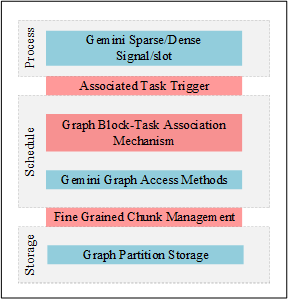
\includegraphics[width=2.5in]{viso插图}
\caption{System Architecture}  
\label{viso插图}
\end{figure}
 
\subsection{Overall Execution Workflow}
We will present the overall execution flow of GraphCPP in pseudo-code. This algorithm takes two input parameters: the set C, containing all graph blocks held by the current computing node, and the set Q, containing all query tasks present on the current computing node. Initially, we allocate a dynamically-sized continuous memory space to store all query tasks (Line 1). Then, we enter a looping process as long as there are unfinished query tasks (Line 2). In this process, GraphCPP calls ChoseNextSharingChunk to select the currently highest-priority graph block, ci. By calculating the associated blocks for each task (i.e., tasks with active vertices in the current block), we identify all query tasks related to the current graph block ci (Line 4). Next, we load ci into the cache and concurrently process all related query operations, qi (Line 5). We invoke GraphCPPCompute to perform the point-to-point query operation qi on the current block. If the query is not yet complete, we update the state of query qi and generate new query tasks (Line 6). If the newly generated query is associated with the current graph block ci, it is added to Qci, and we return to Line 5 to continue querying. Otherwise, the information for the newly generated query is stored in the query task collection, and the task is suspended.

\begin{algorithm}
  \caption{Concurrent Point-to-Point Queries on a Set of Graph Blocks Owned by a Graph Partition}
  \label{algorithm:concurrent-queries}
  \begin{algorithmic}[1]
  \Procedure{MallocBuffers}{$B, Q$} \Comment{B is the set of graph blocks, and Q is the set of query tasks}
      \While{\textsc{has\_active}($B$)}
          \State $bi \gets \text{ChooseNextSharingBlock}()$
          \State $Q_{bi} \gets \text{ChooseAssociatedQueries}(bi)$
          \For{$q_i$ \textbf{in} $Q_{bi}$} \Comment{Execute queries in Q in parallel, which is associated with block $bi$}
              \State $new\_query \gets \text{GraphCPPCompute}(q_i, bi)$ \Comment{The implementation function for point-to-point queries returns the active vertex set after one round of task iteration.}
              \If{\textsc{has\_Associated}($(bi, new\_query)$)}
                  \State $Q_{bi}.\text{Push}(new\_query)$
              \Else
                  \State $Q.\text{Push}(new\_query)$
              \EndIf
          \EndFor
      \EndWhile
  \EndProcedure
  \end{algorithmic}
  \end{algorithm}
  
The above algorithm demonstrates the data sharing mechanism in GraphCPP, with the GraphCPPCompute function utilizing the compute sharing mechanism. The following sections will provide a detailed explanation of these two optimization mechanisms.  

\subsection{Data Access Sharing Mechanism}
In Section 2.2, we observed a significant overlap in the graph structure data access among concurrent tasks. Under the existing processing mechanism, this overlapping data cannot be shared and utilized. However, for point-to-point query tasks on the graph, the order of data access does not affect the correctness of the results. Our data sharing mechanism essentially transforms the original "task → data" linear task scheduling order into a "data → task" fine-grained concurrent task scheduling order, thereby improving cache utilization efficiency and system throughput. To implement this execution model, we need to address two issues: 1) How to determine the shared data segments? 2) How to implement data sharing among multiple tasks? Below are our implementation details.

A. How to Determine Shared Data Segments?

1.Determine the granularity of shared graph data. Distributed memory systems use caching to improve data access efficiency. Ideally, the shared graph partition should be able to fit entirely into the Last Level Cache (LLC), thereby avoiding the frequent swapping in and out of block parts. However, the granularity of graph partition should not be too small, as it would increase the synchronization overhead of task processing. The following demonstrates how to determine an appropriate block size by considering both block-level graph structure data and task-specific data.

We use CS to represent the size of the fine-grained data block to be determined for sharing, and GS to represent the size of the graph structure data on each graph partition. $a$ represents the proportion of the shared block part in the partition image. We use $|V|$ to represent the total number of vertices on the partition. $a*|V|$ represents an approximate value of the number of vertices owned by the shared block. We use VS to represent the average space required to store the status information of a vertex. $a*|V|*V_S$ represents the maximum space required for storing task-specific data on the shared block for query tasks. Considering that multiple cores in multi-core processors execute concurrently, task-specific information for multiple queries needs to be retained in the cache. We use N to represent the number of threads executing parallel computations, and $T_S$ represents the space required to store task-specific data of associated tasks for the current block in the cache. RS is the size of reserved redundant space. LLCS is the size of LLC cache space. Under the premise of satisfying the following inequalities, the maximum value of $C_S$ is the size of the graph block.

2. Logical Partitioning. Distributed systems commonly employ partitioning techniques to divide a large-scale graph into graph partitions that can fit into the memory of a single machine. Building upon the memory-level graph partitioning, GraphCPP further divides the graph into fine-grained graph blocks. Unlike previous physical partitioning, the block partitioning here is based on logical divisions. Pseudocode for partitioning graph blocks in GraphCPP is presented in Listing X:

\begin{algorithm}
\caption{Logical Partition Algorithm}
\begin{algorithmic}[1]
\Function{Partition}{$P_i, B$} \Comment{B is the set of graph blocks owned by graph partition $P_i$.}
    \State $block\_table \gets$ null
    \For{each $e \in P_i$}  \Comment{$e$ is an edge in partition $P_i$}
        \If{$e.src$ in $block\_table$}
            \State $block\_table[e.src] \mathrel{+{+}}$
        \Else
            \State $block\_table[e.src] \gets 1$
        \EndIf
        \If{$\text{block\_table.size()} \geq SC$}
            \State $B.\text{push}(block\_table)$
            \State $block\_table.\text{clear()}$
        \EndIf
    \EndFor
\EndFunction
\end{algorithmic}
\end{algorithm}

Logical Partitioning Function takes two parameters: one is the graph partition structure data Pi recorded in edge table format, and the other is the set of logically divided blocks called $block_set$. Then, define the variable $block_edge_num$ to record the current partition's number of edges. Define the variable block, which is a dictionary with keys representing source vertex IDs, and values representing the number of outgoing edges for each vertex. Iterate through each edge in the partition. If the edge has already been loaded into the current partition, increment the corresponding count of outgoing edges for that partition. If the vertex is added to the block dictionary for the first time, set the count of outgoing edges for the partition to 1. After processing each edge, check if the current block is full. If so, add the current block to $block_set$. This way, after traversing all the data in the partition, every edge in the partition is assigned to a specific graph block, resulting in a set of logically partitioned graph blocks.

3. Associate Query Tasks with Respective Blocks. In the previous step, we achieved fine-grained block partitioning using a logical approach. Since this partitioning is purely logical and the data remains contiguous on the physical storage medium, it becomes straightforward to determine the block a vertex belongs to based on its ID. Specifically, each query task maintains a record of the active vertex set during the traversal process. Initially, we infer the block in which a vertex resides by examining its ID. Subsequently, we employ a specially designed array to store the partitions traversed by each task. Due to the pruning-based traversal strategy employed in point-to-point queries, the number of active vertices in each round of execution is relatively low. This allows us to establish the association between query tasks and their respective blocks at a low cost.

4. Determining Priority for Partition Scheduling. After establishing the association between query tasks and their corresponding blocks, we can tally the number of tasks associated with each block. A higher task count implies that more tasks share this block, indicating a greater benefit derived from scheduling this block. Consequently, such blocks are given priority during scheduling.

Through the aforementioned steps, we generate partitions for task sharing. By employing an economical priority scheduling sequence, we load these graph partitions into the LLC cache. Subsequently, a fine-grained processing mechanism is required to effectively utilize this shared data.

  


  

\section{Where to get the IEEEtran Templates}
\noindent The {\bf{IEEE Template Selector}} will always have the most up-to-date versions of the \LaTeX\ and MSWord templates. Please see: \url{https://template-selector.ieee.org/} and follow the steps to find the correct template for your intended publication. Many publications use the IEEETran LaTeX templates, however, some publications have their own special templates. Many of these are  based on IEEEtran, but may have special instructions that vary slightly from those in this document.

\section{Where to get \LaTeX \ help - user groups}
\noindent The following on-line groups are very helpful to beginning and experienced \LaTeX\ users. A search through their archives can provide many answers to common questions.
\begin{list}{}{}
\item{\url{http://www.latex-community.org/}} 
\item{\url{https://tex.stackexchange.com/} }
\end{list}

\section{Document Class Options in IEEEtran}
\noindent At the beginning of your \LaTeX\ file you will need to establish what type of publication style you intend to use. The following list shows appropriate documentclass options for each of the types covered by IEEEtran.

\begin{list}{}{}
\item{Regular Journal Article}
\item{{\tt{$\backslash$documentclass[journal]{IEEEtran}}}}\\
\item{{Conference Paper}}
\item{{\tt{$\backslash$documentclass[conference]{IEEEtran}}}}\\
\item{Computer Society Journal Article}
\item{{\tt{$\backslash$documentclass[10pt,journal,compsoc]{IEEEtran}}}}\\
\item{Computer Society Conference Paper}
\item{{\tt{$\backslash$documentclass[conference,compsoc]{IEEEtran}}}}\\
\item{{Communications Society Journal Article}}
\item{{\tt{$\backslash$documentclass[journal,comsoc]{IEEEtran}}}}\\
\item{{Brief, Correspondence or Technote}}
\item{{\tt{$\backslash$documentclass[9pt,technote]{IEEEtran}}}}
\end{list}

There are other options available for each of these when submitting for peer review or other special requirements. IEEE recommends to compose your article in the base 2-column format to make sure all your equations, tables and graphics will fit the final 2-column format. Please refer to the document ``IEEEtran\_HOWTO.pdf'' for more information on settings for peer review submission if required by your EIC.

\section{How to Create Common Front Matter}
\noindent The following sections describe general coding for these common elements. Computer Society publications and Conferences may have their own special variations and will be noted below.
\subsection{Paper Title}
\noindent The title of your paper is coded as:

\begin{verbatim}
\title{The Title of Your Paper}
\end{verbatim}

\noindent Please try to avoid the use of math or chemical formulas in your title if possible.

\subsection{Author Names and Affiliations}
\noindent The author section should be coded as follows:
\begin{verbatim}
\author{Masahito Hayashi 
\IEEEmembership{Fellow, IEEE}, Masaki Owari
\thanks{M. Hayashi is with Graduate School 
of Mathematics, Nagoya University, Nagoya, 
Japan}
\thanks{M. Owari is with the Faculty of 
Informatics, Shizuoka University, 
Hamamatsu, Shizuoka, Japan.}
}
\end{verbatim}
Be sure to use the $\backslash$IEEEmembership command to identify IEEE membership status.
Please see the ``IEEEtran\_HOWTO.pdf'' for specific information on coding authors for Conferences and Computer Society publications. Note that the closing curly brace for the author group comes at the end of the thanks group. This will prevent you from creating a blank first page.

\subsection{Running Heads}
\noindent The running heads are declared by using the $\backslash${\tt{markboth}} command. There are two arguments to this command: the first contains the journal name information and the second contains the author names and paper title.
\begin{verbatim}
\markboth{Journal of Quantum Electronics, 
Vol. 1, No. 1, January 2021}
{Author1, Author2, 
\MakeLowercase{\textit{(et al.)}: 
Paper Title}
\end{verbatim}

\subsection{Copyright Line}
\noindent For Transactions and Journals papers, this is not necessary to use at the submission stage of your paper. The IEEE production process will add the appropriate copyright line. If you are writing a conference paper, please see the ``IEEEtran\_HOWTO.pdf'' for specific information on how to code "Publication ID Marks".

\subsection{Abstracts}
\noindent The abstract is the first element of a paper after the $\backslash${\tt{maketitle}} macro is invoked.  The coding is simply:
\begin{verbatim}
\begin{abstract}
Text of your abstract.
\end{abstract}
\end{verbatim}
Please try to avoid mathematical and chemical formulas in the abstract.

\subsection{Index Terms}
\noindent The index terms are used to help other researchers discover your paper. Each society may have it's own keyword set. Contact the EIC of your intended publication for this list.
\begin{verbatim}
\begin{IEEEkeywords}
Broad band networks, quality of service
\end{IEEEkeywords}
\end{verbatim}
\section{How to Create Common Body Elements}
\noindent The following sections describe common body text elements and how to code them.

\subsection{Initial Drop Cap Letter}
\noindent The first text paragraph uses a ``drop cap'' followed by the first word in ALL CAPS. This is accomplished by using the $\backslash${\tt{IEEEPARstart}} command as follows:
\begin{verbatim}
\IEEEPARstart{T}{his} is the first paragraph 
of your paper. . .
\end{verbatim}

\subsection{Sections and Subsections}
\noindent Section headings use standard \LaTeX\ commands: $\backslash${\tt{section}}, $\backslash${\tt{subsection}} and $\backslash${\tt{subsubsection}}. Numbering is handled automatically for you and varies according to type of publication. It is common to not indent the first paragraph following a section head by using $\backslash${\tt{noindent}} as follows:
\begin{verbatim}
\section{Section Head}
\noindent The text of your paragraph . . .
\end{verbatim}

\subsection{Citations to the Bibliography}
\noindent The coding for the citations are made with the \LaTeX\ $\backslash${\tt{cite}} command. This will produce individual bracketed reference numbers in the IEEE style. At the top of your \LaTeX\ file you should include:
\begin{verbatim}
\usepackage{cite}
\end{verbatim}
For a single citation code as follows:
\begin{verbatim}
see \cite{ams}
\end{verbatim}
This will display as: see \cite{ams}\\

For multiple citations code as follows:
\begin{verbatim}
\cite{ams,oxford,lacomp}
\end{verbatim}

This will display as \cite{ams,oxford,lacomp}

\subsection{Figures}
\noindent Figures are coded with the standard \LaTeX\ commands as follows:
\begin{verbatim}
\begin{figure}[!t]
\centering
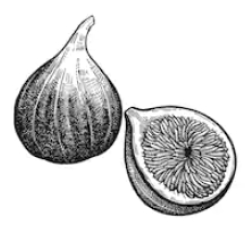
\includegraphics[width=2.5in]{fig1}
\caption{This is the caption for one fig.}
\label{fig1}
\end{figure}
\end{verbatim}
The [!t] argument enables floats to the top of the page to follow IEEE style. Make sure you include:
\begin{verbatim}
\usepackage{graphicx}
\end{verbatim}
 
\noindent at the top of your \LaTeX file with the other package declarations. 

To cross-reference your figures in the text use the following code example:
\begin{verbatim}
See figure \ref{fig1} ...
\end{verbatim}
This will produce:\\
See figure \ref{fig1} . . .

\begin{figure}[!t]
\centering
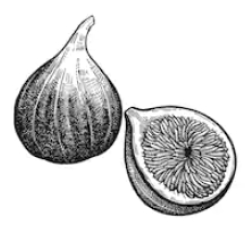
\includegraphics[width=2.5in]{fig1}
\caption{This is the caption for one fig.}
\label{fig1}
\end{figure}

\subsection{Tables}
\noindent Tables should be coded with the standard \LaTeX\ coding. The following example shows a simple table.


\begin{verbatim}
\begin{table}
\begin{center}
\caption{Filter design equations  ...}
\label{tab1}
\begin{tabular}{| c | c | c |}
\hline
Order & Arbitrary coefficients & 
coefficients\\
of filter & $e_m$ &   $b_{ij}$ \\
\hline
1& $b_{ij}=\hat{e}.\hat{\beta_{ij}}$, 
& $b_{00}=0$\\
\hline
2&$\beta_{22}=(~1,-1,-1,~~1,~~1,~~1)$ &\\ 
\hline
3& $b_{ij}=\hat{e}.\hat{\beta_{ij}}$, 
& $b_{00}=0$,\\
\hline 
\end{tabular}
\end{center}
\end{table}
\end{verbatim}
To reference the table in the text, code as follows:
\begin{verbatim}Table~\ref{tab1} lists the closed-form...\end{verbatim}
to produce:

Table~\ref{tab1} lists the closed-form . . .


%moved here for pagination purposes
\begin{table}
\begin{center}
\caption{A Simple Table Example.}
\label{tab1}
\begin{tabular}{| c | c | c |}
\hline
Order & Arbitrary coefficients & coefficients\\
of filter & $e_m$ &   $b_{ij}$ \\
\hline
1& $b_{ij}=\hat{e}.\hat{\beta_{ij}}$, & $b_{00}=0$\\
\hline
2&$\beta_{22}=(~1,-1,-1,~~1,~~1,~~1)$ &\\ 
\hline
3& $b_{ij}=\hat{e}.\hat{\beta_{ij}}$, & $b_{00}=0$,\\
\hline 
\end{tabular}
\end{center}
\end{table}


\subsection{Lists}
\noindent In this section, we will consider three types of lists: simple unnumbered, numbered and bulleted. There have been numerous options added to IEEEtran to enhance the creation of lists. If your lists are more complex than those shown below, please refer to the  ``IEEEtran\_HOWTO.pdf'' for additional options.\\

\noindent{\bf A plain  unnumbered list}

\begin{list}{}{}
\item{bare\_jrnl.tex}
\item{bare\_conf.tex}
\item{bare\_jrnl\_compsoc.tex}
\item{bare\_conf\_compsoc.tex}
\item{bare\_jrnl\_comsoc.tex}
\end{list}

\noindent coded as:
\begin{verbatim}
\begin{list}{}{}
\item{bare\_jrnl.tex}
\item{bare\_conf.tex}
\item{bare\_jrnl\_compsoc.tex}
\item{bare\_conf\_compsoc.tex}
\item{bare\_jrnl\_comsoc.tex}
\end{list}
\end{verbatim}
\noindent{\bf A simple numbered list}

\begin{enumerate}
\item{bare\_jrnl.tex}
\item{bare\_conf.tex}
\item{bare\_jrnl\_compsoc.tex}
\item{bare\_conf\_compsoc.tex}
\item{bare\_jrnl\_comsoc.tex}
\end{enumerate}
\noindent coded as: 
\begin{verbatim}
\begin{enumerate}
\item{bare\_jrnl.tex}
\item{bare\_conf.tex}
\item{bare\_jrnl\_compsoc.tex}
\item{bare\_conf\_compsoc.tex}
\item{bare\_jrnl\_comsoc.tex}
\end{enumerate}
\end{verbatim}

\noindent{\bf A simple bulleted list}

\begin{itemize}
\item{bare\_jrnl.tex}
\item{bare\_conf.tex}
\item{bare\_jrnl\_compsoc.tex}
\item{bare\_conf\_compsoc.tex}
\item{bare\_jrnl\_comsoc.tex}
\end{itemize}

\noindent coded as:

\begin{verbatim}
\begin{itemize}
\item{bare\_jrnl.tex}
\item{bare\_conf.tex}
\item{bare\_jrnl\_compsoc.tex}
\item{bare\_conf\_compsoc.tex}
\item{bare\_jrnl\_comsoc.tex}
\end{itemize}
\end{verbatim}


\subsection{Other Elements}
\noindent For other less common elements such as Algorithms, Theorems and Proofs, and Floating Structures such as page-wide tables, figures or equations, please refer to the ``IEEEtran\_HOWTO.pdf'' section on ``Double Column Floats.''


\section{How to Create Common Back Matter Elements}
\noindent The following sections demonstrate common back matter elements such as Acknowledgments, Bibliographies, Appendicies and Author Biographies.

\subsection{Acknowledgments}
\noindent This should be a simple paragraph before the bibliography to thank those individuals and institutions who have supported your work on this article.

\begin{verbatim}
\section{Acknowledgments}
\noindent Text describing those who 
supported your paper.
\end{verbatim}

\subsection{Bibliographies}
\noindent {\bf{References Simplified:}} A simple way of composing references is to use the $\backslash${\tt{bibitem}} macro to define the beginning of a reference as in the following examples:\\


\noindent [6] H. Sira-Ramirez. ``On the sliding mode control of nonlinear systems,'' \textit{Systems \& Control Letters}, vol. 19, pp. 303--312, 1992.

\noindent coded as:
\begin{verbatim}
\bibitem{Sira3}
H. Sira-Ramirez. ``On the sliding mode 
control of nonlinear systems,'' 
\textit{Systems \& Control Letters}, 
vol. 19, pp. 303--312, 1992.
\end{verbatim}

\noindent [7] A. Levant.``Exact differentiation of signals with unbounded higher derivatives,''  in \textit{Proceedings of the 45th IEEE Conference on Decision and Control}, San Diego, California, USA, pp. 5585--5590, 2006.

\noindent coded as:
\begin{verbatim}\bibitem{Levant}
A. Levant. ``Exact differentiation of 
signals with unbounded higher 
derivatives,''  in \textit{Proceedings 
of the 45th IEEE Conference on 
Decision and Control}, San Diego, 
California, USA, pp. 5585--5590, 2006.
\end{verbatim}


\noindent [8] M. Fliess, C. Join, and H. Sira-Ramirez. ``Non-linear estimation is easy,'' \textit{International Journal of Modelling, Identification and Control}, vol. 4, no. 1, pp. 12--27, 2008.

\noindent coded as:
\begin{verbatim}
\bibitem{Cedric}
M. Fliess, C. Join, and H. Sira-Ramirez. 
``Non-linear estimation is easy,'' 
\textit{International Journal of Modelling, 
Identification and Control}, vol. 4, 
no. 1, pp. 12--27, 2008.
\end{verbatim}

\noindent [9] R. Ortega, A. Astolfi, G. Bastin, and H. Rodriguez. ``Stabilization of food-chain systems using a port-controlled Hamiltonian description,'' in \textit{Proceedings of the American Control Conference}, Chicago, Illinois, USA, pp. 2245--2249, 2000.

\noindent coded as:
\begin{verbatim}
\bibitem{Ortega}
R. Ortega, A. Astolfi, G. Bastin, and H. 
Rodriguez. ``Stabilization of food-chain 
systems using a port-controlled Hamiltonian 
description,'' in \textit{Proceedings of the 
American Control Conference}, Chicago, 
Illinois, USA, pp. 2245--2249, 2000.
\end{verbatim}

\subsection{Accented Characters in References}
\noindent When using accented characters in references, please use the standard LaTeX coding for accents. {\bf{Do not use math coding for character accents}}. For example:
\begin{verbatim}
\'e, \"o, \`a, \~e 
\end{verbatim}
will produce: \'e, \"o, \`a, \~e 


\subsection{Use of BibTeX}
\noindent If you wish to use BibTeX, please see the documentation that accompanies the IEEEtran Bibliography package.

\subsection{Biographies and Author Photos}
\noindent Authors may have options to include their photo or not. Photos should be a bit-map graphic (.tif or .jpg) and sized to fit in the space allowed. Please see the coding samples below:
\begin{verbatim}
\begin{IEEEbiographynophoto}{Jane Doe}
Biography text here without a photo.
\end{IEEEbiographynophoto}
\end{verbatim}
or a biography with a photo

\begin{verbatim}
\begin{IEEEbiography}[{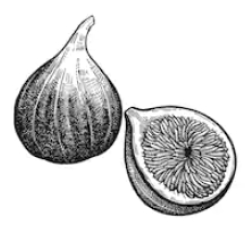
\includegraphics
[width=1in,height=1.25in,clip,
keepaspectratio]{fig1.png}}]
{IEEE Publications Technology Team} 
In this paragraph you can place 
your educational, professional background 
and research and other interests.
\end{IEEEbiography}
\end{verbatim}

Please see the end of this document to see the output of these coding examples.



\section{Mathematical Typography \\ and Why It Matters}

\noindent Typographical conventions for mathematical formulas have been developed to {\bf provide uniformity and clarity of presentation across mathematical texts}. This enables the readers of those texts to both understand the author's ideas and to grasp new concepts quickly. While software such as \LaTeX \ and MathType\textsuperscript{\textregistered} can produce aesthetically pleasing math when used properly, it is also very easy to misuse the software, potentially resulting in incorrect math display.

IEEE aims to provide authors with the proper guidance on mathematical typesetting style and assist them in writing the best possible article.

As such, IEEE has assembled a set of examples of good and bad mathematical typesetting. You will see how various issues are dealt with. The following publications have been referenced in preparing this material:

\begin{list}{}{}
\item{\emph{Mathematics into Type}, published by the American Mathematical Society}
\item{\emph{The Printing of Mathematics}, published by Oxford University Press}
\item{\emph{The \LaTeX Companion}, by F. Mittelbach and M. Goossens}
\item{\emph{More Math into LaTeX}, by G. Gr\"atzer}
\item{AMS-StyleGuide-online.pdf, published by the American Mathematical Society}
\end{list}

Further examples can be seen at \url{http://journals.ieeeauthorcenter.ieee.org/wp-content/uploads/sites/7/IEEE-Math-Typesetting-Guide.pdf}

\subsection{Display Equations}
\noindent A simple display equation example shown below uses the ``equation'' environment. To number the equations, use the $\backslash${\tt{label}} macro to create an identifier for the equation. LaTeX will automatically number the equation for you.
\begin{equation}
\label{deqn_ex1}
x = \sum_{i=0}^{n} 2{i} Q.
\end{equation}

\noindent is coded as follows:
\begin{verbatim}
\begin{equation}
\label{deqn_ex1}
x = \sum_{i=0}^{n} 2{i} Q.
\end{equation}
\end{verbatim}

To reference this equation in the text use the $\backslash${\tt{ref}} macro. 
Please see (\ref{deqn_ex1})\\
\noindent is coded as follows:
\begin{verbatim}
Please see (\ref{deqn_ex1})\end{verbatim}

\subsection{Equation Numbering}
\noindent {\bf{Consecutive Numbering:}} Equations within an article are numbered consecutively from the beginning of the
article to the end, i.e., (1), (2), (3), (4), (5), etc. Do not use roman numerals or section numbers for equation numbering.\\

\noindent {\bf{Appendix Equations:}} The continuation of consecutively numbered equations is best in the Appendix, but numbering
 as (A1), (A2), etc., is permissible.\\

\noindent {\bf{Hyphens and Periods}}: Hyphens and periods should not be used in equation numbers, i.e., use (1a) rather than
(1-a) and (2a) rather than (2.a) for sub-equations. This should be consistent throughout the article.

\subsection{Multi-line equations and alignment}
\noindent Here we show several examples of multi-line equations and proper alignments.

\noindent {\bf{A single equation that must break over multiple lines due to length with no specific alignment.}}
\begin{multline}
\text{The first line of this example}\\
\text{The second line of this example}\\
\text{The third line of this example}
\end{multline}

\noindent is coded as:
\begin{verbatim}
\begin{multline}
\text{The first line of this example}\\
\text{The second line of this example}\\
\text{The third line of this example}
\end{multline}
\end{verbatim}

\noindent {\bf{A single equation with multiple lines aligned at the = signs}}
\begin{align}
a &= c+d \\
b &= e+f
\end{align}
\noindent is coded as:
\begin{verbatim}
\begin{align}
a &= c+d \\
b &= e+f
\end{align}
\end{verbatim}

The {\tt{align}} environment can align on multiple  points as shown in the following example:
\begin{align}
x &= y & X & =Y & a &=bc\\
x' &= y' & X' &=Y' &a' &=bz
\end{align}
\noindent is coded as:
\begin{verbatim}
\begin{align}
x &= y & X & =Y & a &=bc\\
x' &= y' & X' &=Y' &a' &=bz
\end{align}
\end{verbatim}





\subsection{Subnumbering}
\noindent The amsmath package provides a {\tt{subequations}} environment to facilitate subnumbering. An example:

\begin{subequations}\label{eq:2}
\begin{align}
f&=g \label{eq:2A}\\
f' &=g' \label{eq:2B}\\
\mathcal{L}f &= \mathcal{L}g \label{eq:2c}
\end{align}
\end{subequations}

\noindent is coded as:
\begin{verbatim}
\begin{subequations}\label{eq:2}
\begin{align}
f&=g \label{eq:2A}\\
f' &=g' \label{eq:2B}\\
\mathcal{L}f &= \mathcal{L}g \label{eq:2c}
\end{align}
\end{subequations}

\end{verbatim}

\subsection{Matrices}
\noindent There are several useful matrix environments that can save you some keystrokes. See the example coding below and the output.

\noindent {\bf{A simple matrix:}}
\begin{equation}
\begin{matrix}  0 &  1 \\ 
1 &  0 \end{matrix}
\end{equation}
is coded as:
\begin{verbatim}
\begin{equation}
\begin{matrix}  0 &  1 \\ 
1 &  0 \end{matrix}
\end{equation}
\end{verbatim}

\noindent {\bf{A matrix with parenthesis}}
\begin{equation}
\begin{pmatrix} 0 & -i \\
 i &  0 \end{pmatrix}
\end{equation}
is coded as:
\begin{verbatim}
\begin{equation}
\begin{pmatrix} 0 & -i \\
 i &  0 \end{pmatrix}
\end{equation}
\end{verbatim}

\noindent {\bf{A matrix with square brackets}}
\begin{equation}
\begin{bmatrix} 0 & -1 \\ 
1 &  0 \end{bmatrix}
\end{equation}
is coded as:
\begin{verbatim}
\begin{equation}
\begin{bmatrix} 0 & -1 \\ 
1 &  0 \end{bmatrix}
\end{equation}
\end{verbatim}

\noindent {\bf{A matrix with curly braces}}
\begin{equation}
\begin{Bmatrix} 1 &  0 \\ 
0 & -1 \end{Bmatrix}
\end{equation}
is coded as:
\begin{verbatim}
\begin{equation}
\begin{Bmatrix} 1 &  0 \\ 
0 & -1 \end{Bmatrix}
\end{equation}\end{verbatim}

\noindent {\bf{A matrix with single verticals}}
\begin{equation}
\begin{vmatrix} a &  b \\ 
c &  d \end{vmatrix}
\end{equation}
is coded as:
\begin{verbatim}
\begin{equation}
\begin{vmatrix} a &  b \\ 
c &  d \end{vmatrix}
\end{equation}\end{verbatim}

\noindent {\bf{A matrix with double verticals}}
\begin{equation}
\begin{Vmatrix} i &  0 \\ 
0 & -i \end{Vmatrix}
\end{equation}
is coded as:
\begin{verbatim}
\begin{equation}
\begin{Vmatrix} i &  0 \\ 
0 & -i \end{Vmatrix}
\end{equation}\end{verbatim}

\subsection{Arrays}
\noindent The {\tt{array}} environment allows you some options for matrix-like equations. You will have to manually key the fences, but you'll have options for alignment of the columns and for setting horizontal and vertical rules. The argument to {\tt{array}} controls alignment and placement of vertical rules.

A simple array
\begin{equation}
\left(
\begin{array}{cccc}
a+b+c & uv & x-y & 27\\
a+b & u+v & z & 134
\end{array}\right)
\end{equation}
is coded as:
\begin{verbatim}
\begin{equation}
\left(
\begin{array}{cccc}
a+b+c & uv & x-y & 27\\
a+b & u+v & z & 134
\end{array} \right)
\end{equation}
\end{verbatim}

A slight variation on this to better align the numbers in the last column
\begin{equation}
\left(
\begin{array}{cccr}
a+b+c & uv & x-y & 27\\
a+b & u+v & z & 134
\end{array}\right)
\end{equation}
is coded as:
\begin{verbatim}
\begin{equation}
\left(
\begin{array}{cccr}
a+b+c & uv & x-y & 27\\
a+b & u+v & z & 134
\end{array} \right)
\end{equation}
\end{verbatim}

An array with vertical and horizontal rules
\begin{equation}
\left( \begin{array}{c|c|c|r}
a+b+c & uv & x-y & 27\\ \hline
a+b & u+v & z & 134
\end{array}\right)
\end{equation}
is coded as:
\begin{verbatim}
\begin{equation}
\left(
\begin{array}{c|c|c|r}
a+b+c & uv & x-y & 27\\
a+b & u+v & z & 134
\end{array} \right)
\end{equation}
\end{verbatim}
Note the argument now has the pipe "$\vert$" included to indicate the placement of the vertical rules.


\subsection{Cases Structures}
\noindent Many times we find cases coded using the wrong environment, i.e., {\tt{array}}. Using the {\tt{cases}} environment will save keystrokes (from not having to type the $\backslash${\tt{left}}$\backslash${\tt{lbrace}}) and automatically provide the correct column alignment.
\begin{equation*}
{z_m(t)} = \begin{cases}
1,&{\text{if}}\ {\beta }_m(t) \\ 
{0,}&{\text{otherwise.}} 
\end{cases}
\end{equation*}
\noindent is coded as follows:
\begin{verbatim}
\begin{equation*}
{z_m(t)} = 
\begin{cases}
1,&{\text{if}}\ {\beta }_m(t),\\ 
{0,}&{\text{otherwise.}} 
\end{cases}
\end{equation*}
\end{verbatim}
\noindent Note that the ``\&'' is used to mark the tabular alignment. This is important to get  proper column alignment. Do not use $\backslash${\tt{quad}} or other fixed spaces to try and align the columns. Also, note the use of the $\backslash${\tt{text}} macro for text elements such as ``if'' and ``otherwise''.

\subsection{Function Formatting in Equations}
In many cases there is an easy way to properly format most common functions. Use of the $\backslash$ in front of the function name will in most cases, provide the correct formatting. When this does not work, the following example provides a solution using the $\backslash${\tt{text}} macro.

\begin{equation*} 
  d_{R}^{KM} = \underset {d_{l}^{KM}} {\text{arg min}} \{ d_{1}^{KM},\ldots,d_{6}^{KM}\}.
\end{equation*}

\noindent is coded as follows:
\begin{verbatim}
\begin{equation*} 
 d_{R}^{KM} = \underset {d_{l}^{KM}} 
 {\text{arg min}} \{ d_{1}^{KM},
 \ldots,d_{6}^{KM}\}.
\end{equation*}
\end{verbatim}

\subsection{ Text Acronyms inside equations}
\noindent This example shows where the acronym ``MSE" is coded using $\backslash${\tt{text\{\}}} to match how it appears in the text.

\begin{equation*}
 \text{MSE} = \frac {1}{n}\sum _{i=1}^{n}(Y_{i} - \hat {Y_{i}})^{2}
\end{equation*}

\begin{verbatim}
\begin{equation*}
 \text{MSE} = \frac {1}{n}\sum _{i=1}^{n}
(Y_{i} - \hat {Y_{i}})^{2}
\end{equation*}
\end{verbatim}

\subsection{Obsolete Coding}
\noindent Avoid the use of outdated environments, such as {\tt{eqnarray}} and \$\$ math delimiters, for display equations. The \$\$ display math delimiters are left over from PlainTeX and should not be used in \LaTeX, ever. Poor vertical spacing will result.
\subsection{Use Appropriate Delimiters for Display Equations}
\noindent Some improper mathematical coding advice has been given in various YouTube\textsuperscript{TM} videos on how to write scholarly articles, so please follow these good examples:\\

For {\bf{single-line unnumbered display equations}}, please use the following delimiters: 
\begin{verbatim}\[ . . . \] or \end{verbatim} 
\begin{verbatim}\begin{equation*} . . . \end{equation*}\end{verbatim}
Note that the * in the environment name turns off equation numbering.\\

For {\bf{multiline unnumbered display equations}} that have alignment requirements, please use the following delimiters: 
\begin{verbatim}
\begin{align*} . . . \end{align*}
\end{verbatim}

For {\bf{single-line numbered display equations}}, please use the following delimiters: 
\begin{verbatim}
\begin{equation} . . . \end{equation}
\end{verbatim}

For {\bf{multiline numbered display equations}}, please use the following delimiters: 
\begin{verbatim}
\begin{align} . . . \end{align}
\end{verbatim}

\section{LaTeX Package Suggestions}
\noindent Immediately after your documenttype declaration at the top of your \LaTeX\ file is the place where you should declare any packages that are being used. The following packages were used in the production of this document.
\begin{verbatim}
\usepackage{amsmath,amsfonts}
% \usepackage{algorithmic}
\usepackage{array}
\usepackage[caption=false,font=normalsize,
   labelfont=sf,textfont=sf]{subfig}
\u00sepackage{textcomp}
\usepackage{stfloats}
\usepackage{url}
\usepackage{verbatim}
\usepackage{graphicx}
\usepackage{balance}
\end{verbatim}

\section{Additional Advice}

Please use ``soft'' (e.g., \verb|\eqref{Eq}|) or \verb|(\ref{Eq})|
cross references instead of ``hard'' references (e.g., \verb|(1)|).
That will make it possible to combine sections, add equations, or
change the order of figures or citations without having to go through
the file line by line.

Please note that the \verb|{subequations}| environment in {\LaTeX}
will increment the main equation counter even when there are no
equation numbers displayed. If you forget that, you might write an
article in which the equation numbers skip from (17) to (20), causing
the copy editors to wonder if you've discovered a new method of
counting.

{\BibTeX} does not work by magic. It doesn't get the bibliographic
data from thin air but from .bib files. If you use {\BibTeX} to produce a
bibliography you must send the .bib files. 

{\LaTeX} can't read your mind. If you assign the same label to a
subsubsection and a table, you might find that Table I has been cross
referenced as Table IV-B3. 

{\LaTeX} does not have precognitive abilities. If you put a
\verb|\label| command before the command that updates the counter it's
supposed to be using, the label will pick up the last counter to be
cross referenced instead. In particular, a \verb|\label| command
should not go before the caption of a figure or a table.

Please do not use \verb|\nonumber| or \verb|\notag| inside the
\verb|{array}| environment. It will not stop equation numbers inside
\verb|{array}| (there won't be any anyway) and it might stop a wanted
equation number in the surrounding equation.

\balance

\section{A Final Checklist}
\begin{enumerate}{}{}  %
\item{Make sure that your equations are numbered sequentially and there are no equation numbers missing or duplicated. Avoid hyphens and periods in your equation numbering. Stay with IEEE style, i.e., (1), (2), (3) or for sub-equations (1a), (1b). For equations in the appendix (A1), (A2), etc.}. 
\item{Are your equations properly formatted? Text, functions, alignment points in cases and arrays, etc. }
\item{Make sure all graphics are included.}
\item{Make sure your references are included either in your main LaTeX file or a separate .bib file if calling the external file.}
\end{enumerate}

\begin{thebibliography}{1} %这里的1是指用最多的数字有几位,比如10就是指用最多的数字有两位

\bibitem{ams} %这行是指把这个参考文献标签为ams,这个标签可以自己取,作用是在正文中引用时用的
{\it{Mathematics into Type}}, American Mathematical Society. Online available:  %\it的意思是把后面的内容变成斜体

\bibitem{oxford} %这行是指把这个参考文献标签为oxford
T.W. Chaundy, P.R. Barrett and C. Batey, {\it{The Printing of Mathematics}}, Oxford University Press. London, 1954.

\bibitem{lacomp}{\it{The \LaTeX Companion}}, by F. Mittelbach and M. Goossens

\bibitem{mmt}{\it{More Math into LaTeX}}, by G. Gr\"atzer

\bibitem{amstyle}{\it{AMS-StyleGuide-online.pdf,}} published by the American Mathematical Society

\bibitem{Sira3}
H. Sira-Ramirez. ``On the sliding mode control of nonlinear systems,'' \textit{Systems \& Control Letters}, vol. 19, pp. 303--312, 1992.

\bibitem{Levant}
A. Levant. ``Exact differentiation of signals with unbounded higher derivatives,''  in \textit{Proceedings of the 45th IEEE Conference on Decision and Control}, San Diego, California, USA, pp. 5585--5590, 2006.

\bibitem{Cedric}
M. Fliess, C. Join, and H. Sira-Ramirez. ``Non-linear estimation is easy,'' \textit{International Journal of Modelling, Identification and Control}, vol. 4, no. 1, pp. 12--27, 2008.

\bibitem{Ortega}
R. Ortega, A. Astolfi, G. Bastin, and H. Rodriguez. ``Stabilization of food-chain systems using a port-controlled Hamiltonian description,'' in \textit{Proceedings of the American Control Conference}, Chicago, Illinois, USA, pp. 2245--2249, 2000. %这里的\textit是指把后面的内容变成斜体

\end{thebibliography} %这个是参考文献的结束

\begin{IEEEbiographynophoto}{Jane Doe} %这里的Jane Doe是指作者的名字
Biography text here without a photo.
\end{IEEEbiographynophoto} %这个是作者的结束

\begin{IEEEbiography}[{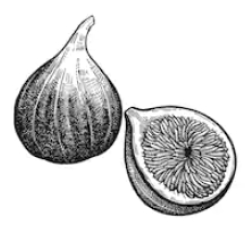
\includegraphics[width=1in,height=1.25in,clip,keepaspectratio]{fig1.png}}]{IEEE Publications Technology Team}
In this paragraph you can place your educational, professional background and research and other interests.\end{IEEEbiography} %这行的作用是插入作者的照片


\end{document}


